% ****** Start of file apssamp.tex ******
%
%   This file is part of the APS files in the REVTeX 4.1 distribution.
%   Version 4.1r of REVTeX, August 2010
%
%   Copyright (c) 2009, 2010 The American Physical Society.
%
%   See the REVTeX 4 README file for restrictions and more information.
%
% TeX'ing this file requires that you have AMS-LaTeX 2.0 installed
% as well as the rest of the prerequisites for REVTeX 4.1
%
% See the REVTeX 4 README file
% It also requires running BibTeX. The commands are as follows:
%
%  1)  latex apssamp.tex
%  2)  bibtex apssamp
%  3)  latex apssamp.tex
%  4)  latex apssamp.tex
%
\documentclass[%
reprint,
%superscriptaddress,
%groupedaddress,
%unsortedaddress,
%runinaddress,
%frontmatterverbose,
%preprint,
%showpacs,preprintnumbers,
%nofootinbib,
%nobibnotes,
%bibnotes,
 amsmath,amssymb,
 %aps,
 prd,
%linenumbers,
%pra,
%prb,
%rmp,
%prstab,
%prstper,
%floatfix,
]{revtex4-1}

\usepackage{graphicx}% Include figure files

%\usepackage{subcaption}
%\usepackage[caption=false]{subfig}

\usepackage{dcolumn}% Align table columns on decimal point
\usepackage{bm}% bold math
%\usepackage{hyperref}% add hypertext capabilities
%\usepackage[mathlines]{lineno}% Enable numbering of text and display math
%\linenumbers\relax % Commence numbering lines

%\usepackage[showframe,%Uncomment any one of the following lines to test
%%scale=0.7, marginratio={1:1, 2:3}, ignoreall,% default settings
%%text={7in,10in},centering,
%%margin=1.5in,
%%total={6.5in,8.75in}, top=1.2in, left=0.9in, includefoot,
%%height=10in,a5paper,hmargin={3cm,0.8in},
%]{geometry}


%%%%%%%%%%%%%%%%%%%%%%%%%%%
%%%%%%  PREAMBLES %%%%%%%%%
\newcommand{\ud}[1]{{#1^{\dagger}}}
\newcommand{\bra}[1]{\left\langle #1\right|}
\newcommand{\ket}[1]{\left| #1\right\rangle}
\newcommand\Tr{\mathrm{Tr}}
\newcommand{\braket}[2]{\langle #1 \mid #2 \rangle}
\newcommand\I{\mathbb{I}}
\newcommand{\avg}[1]{\left< #1 \right>}
\newcommand{\sech}[1]{{\operatorname{sech}{#1}}}
\newcommand{\csch}[1]{{\operatorname{csch}{#1}}}
\newcommand{\RD}{D}
\newcommand{\ri}{\mathrm{i}}
\DeclareMathOperator{\sign}{sign}

%%%%%%  PREAMBLES %%%%%%%%%
%%%%%%%%%%%%%%%%%%%%%%%%%%%

\begin{document}

%\preprint{APS/123-QED}

\title{Parametric neutrino flavor conversions and Rabi oscillations}% Force line breaks with \\
%\thanks{A footnote to the article title}%

\author{Lei Ma}
\email{leima@unm.edu}
\author{Shashank Shalgar}%
\email{shashankshalgar@unm.edu}
\author{Huaiyu Duan}%
\email{duan@unm.edu}
\affiliation{%
 Department of Physics \& Astronomy, University of New Mexico,
 Albuquerque, NM 87131, USA
}%
% \author{Huaiyu Duan}%
%  \email{Second.Author@institution.edu}
% \affiliation{%
%  Authors' institution and/or address\\
%  This line break forced with \textbackslash\textbackslash
% }%

% \collaboration{MUSO Collaboration}%\noaffiliation

% \author{Shashank Shalgar}
%  \homepage{http://www.Second.institution.edu/~Charlie.Author}
% \affiliation{
%  Second institution and/or address\\
%  This line break forced% with \\
% }%
% \affiliation{
%  Third institution, the second for Charlie Author
% }%
% \author{Delta Author}
% \affiliation{%
%  Authors' institution and/or address\\
%  This line break forced with \textbackslash\textbackslash
% }%

% \collaboration{CLEO Collaboration}%\noaffiliation

% \author{Huaiyu Duan}
%  \homepage{http://www.Second.institution.edu/~Charlie.Author}
% \affiliation{
%  Second institution and/or address\\
%  This line break forced% with \\
% }%
% \affiliation{
%  Third institution, the second for Charlie Author
% }%
% \author{Delta Author}
% \affiliation{%
%  Authors' institution and/or address\\
%  This line break forced with \textbackslash\textbackslash
% }%

% \collaboration{CLEO Collaboration}%\noaffiliation



\date{\today}% It is always \today, today,
             %  but any date may be explicitly specified

\begin{abstract}

We develop an interpretation of neutrino flavor conversions in fluctuating matter density based on Rabi oscillations. In certain limits, matter density fluctuations with single frequency modulates the neutrino flavor conversion similar to Rabi oscillations in optics. Adding more frequencies in matter fluctuations have complicated effects on the neutrino flavor conversions, which is interference between each frequencies. The interference is explored and criteria of interference is proposed and verified numerically. By switching to a new basis, we are able to expand neutrino flavor conversions in matter with multiple-frequency fluctuations into superposition of Rabi oscillations. Using this technique we explain the relation between neutrino flavor conversions and Rabi oscillations by taking into account of the interference between different modes of Rabi oscillations more quantitatively.

% \fbox{ABSTRACT PLACEHOLDER}
% \begin{description}
% \item[Usage]
% Secondary publications and information retrieval purposes.
% \item[PACS numbers]
% May be entered using the \verb+\pacs{#1}+ command.
% \item[Structure]
% You may use the \texttt{description} environment to structure your abstract;
% use the optional argument of the \verb+\item+ command to give the category of each item.
% \end{description}
\end{abstract}

% \pacs{Valid PACS appear here}% PACS, the Physics and Astronomy
                             % Classification Scheme.
%\keywords{Suggested keywords}%Use showkeys class option if keyword
                              %display desired
\maketitle

%\tableofcontents

\section{\label{introduction}Introduction}

In many astrophysical environments, such as core-collapse supernova,  neutrinos propagate through dense fluctuating medium, which will interact with neutrinos and dramatically change the flavor oscillations of neutrinos. Meanwhile, neutrinos deposit energy in matter during the interaction, where the amount of energy deposited depends on the flavor of neutrinos. The significance of matter effect on neutrino flavor oscillations has been demonstrated in Mikheyev–-Smirnov–-Wolfenstein (MSW) effect~\cite{Mikheev:1986gs,wolf78,wolfensteinprd1979}, which is used to explain the deficit of electron flavor neutrino flux, thus solved the solar neutrino problem~\cite{Petcov2002,kuo1989}. Later developments on the theories about matter effect revealed the parametric resonance of neutrino flavor oscillations due to fluctuations in matter density~\cite{Krastev1989,Akhmedov2000}, which is the neutrino analog of transitions between energy levels as a result of external optical stimulation. Parametric resonance is different from the MSW effect since it involves the parameters of the matter density, which is usually the period of matter density fluctuations. Neutrinos passing through inside the Earth can experience parametric resonance~\cite{Akhmedov1999, Petcov1998b}.

As one of the most intense neutrino sources, supernova neutrinos experience turbulent matter density as they propagate through out the explosion~\cite{Muller2015, Couch2015}, where the flavor conversion is modified by interaction with matter. Meanwhile with neutrinos depositing energy into the shock, neutrino flavor conversion is crucial to the shock evolution of supernova explosion. The turbulent matter density environment for neutrino flavor conversion has been researched~\cite{Loreti1994, Friedland2006,Kneller2010}. Recently matter stimulated neutrino flavor conversion in varying matter density has been researched using Jacobi-Anger expansion by Kneller, et al.~\cite{Kneller2013,Patton2014}. They have shown that many stimulated neutrino flavor conversions can be explained by resonances of the system.

In this paper, we take a step further and interpret parametric resonance~\cite{Akhmedov2000, Krastev1989} as well as other matter stimulated neutrino flavor conversions~\cite{Kneller2013, Patton2014}, as superposition of Rabi oscillations. We also propose a criteria for the interference effect between different Rabi oscillations modes. In Sec.~\ref{sec:background}, we define the formalism of neutrino flavor conversions in matter used in this paper where the equation of motion and Hamiltonian for neutrino flavor conversion in matter are explicitly written. In Sec.~\ref{sec:single} we discuss how neutrino flavor conversions are related to Rabi oscillations. To begin with, we discuss a system with single frequency matter density fluctuation. We will show that such a system can be reduced to Rabi oscillations if resonance occurs. In Sec.~\ref{sec:multiple} we describe the interference effect between different frequencies of Rabi oscillations and develop the criteria for significant interference between two frequencies. We show that the interference between the many frequencies fits into the criteria we proposed for interference. In Sec.~\ref{sec:jacobi} we discuss the technique of decomposing the neutrino flavor conversions into summation of Rabi oscillations, by applying a specific unitary transformation and the Jacobi-Anger expansion. As the system is exactly decomposed into multiple Rabi oscillations, we can interpret neutrino flavor oscillations in any matter density fluctuations in principle. As an example, we solve the neutrino flavor transitions in a castle wall matter profile, which is expanded using Fourier series into many frequencies.


% \fbox{TODO:more about oscillation in matter}

\section{\label{sec:background}Background and Formalism}

% \fbox{TODO: Explain why two flavor} didn't add this because the three flavor is really very different.

We consider two-flavor oscillation scenario, in which neutrinos have energy $E$ and mass-squared difference $\delta m^2$ between two mass states propagate through matter which is define by electron number density profile $n(r)$ along the path of neutrino propagation $r$.  The dynamics of neutrino flavor conversion is determined by Schr\"{o}dinger equation. In flavor basis the wave function describes the probability amplitude of different flavors. The Hamiltonian in flavor basis consists the vacuum oscillation Hamiltonian $H^{(f)}_{\mathrm v}$ and the matter term $H^{(f)}_{\mathrm{m}}$ which describes the interaction between neutrinos and matter,
\begin{align}
    H^{(\mathrm{f})} =&  H^{(f)}_{\mathrm v} + H^{(f)}_{\mathrm m} \nonumber\\
    =&  \frac{1}{2} \begin{pmatrix}
    -\omega_{\mathrm{v}} \cos 2\theta_{\mathrm{v}} + \lambda(r) & \omega_{\mathrm{v}}\sin 2\theta_{\mathrm{v}} \\
   \omega_{\mathrm{v}} \sin 2\theta_{\mathrm{v}} & \omega_{\mathrm{v}} \cos 2\theta_{\mathrm{v}} - \lambda(r)
    \end{pmatrix},
\end{align}
where $\lambda(r)= \sqrt{2}G_{\mathrm F} n(r)$ is the potential of neutrino interaction with matter and $G_{\mathrm F}$ is the Fermi constant, $\theta_{\mathrm{v}}$ is the vacuum mixing angle, $\omega_{\mathrm{v}} = \delta m^2/2E$ is the vacuum oscillation frequency. The potential $\lambda(r)$ is called matter profile since it reflects the matter density fluctuations. For the convenience of notation, we use Pauli matrices $\sigma_i$ to rewrite the Hamiltonian, so that the Schr\"{o}dinger equation becomes,
\begin{equation*}
    \mathrm i\frac{\mathrm d}{\mathrm d r}\Psi(r) = \frac{1}{2} \left(
    (- \omega_{\mathrm{v}}\cos 2\theta_{\mathrm{v}} + \lambda(r) ) \sigma_3 + \omega_{\mathrm{v}}\sin 2\theta_{\mathrm{v}} \sigma_1
    \right)
    \Psi(r),
\end{equation*}
where $\Psi(r)$ is the wave function in flavor basis. For two flavor scenario, it is written as $ \Psi(r) = \left(
    \psi_{e} ,
    \psi_{x}
    \right)^{\mathrm{T}}$
where $\psi_{e}$ and $\psi_{x}$ are the amplitudes for electron flavor and the second flavor ($\mu$ flavor or $\tau$ flavor) respectively. The equation of motion in flavor basis governs the transitions between different flavors.

For arbitrary matter profile, we can always interpret it as perturbations on top of a constant matter profile,
\begin{equation}
    \lambda(r) = \lambda_0 + \delta \lambda(r).
    \label{eq-general-matter-profile}
\end{equation}
For better understanding of the transition between states as a consequence of the fluctuation of matter density, we use the background matter basis, in which the Hamiltonian is diagonalized in the absence of perturbation $\delta\lambda(r)$, so that the Hamiltonian reads
\begin{widetext}
\begin{equation}
    H^{(\mathrm{m})} = -\frac{\omega_m}{2} \sigma_3 + \frac{1}{2} \delta\lambda(r) \cos 2\theta_{\mathrm m} \sigma_3
     - \frac{1}{2} \delta\lambda(r) \sin 2\theta_{\mathrm m} \sigma_1,
    \label{eq-hamiltonian-bg-matter-basis-general}
\end{equation}
\end{widetext}
where $\theta_{\mathrm m}$ is the mixing angle in a constant matter profile $\lambda_0$, which is calculated using relation
\begin{equation*}
\tan 2\theta_{\mathrm{m}}=\sin 2\theta_{\mathrm v}/\left( \cos 2\theta_{\mathrm v} - \lambda_0/\omega_{\mathrm v} \right)
\end{equation*}
with $\omega_{\mathrm v}$ denoting the vacuum oscillation frequency and $\theta_{\mathrm v}$ denoting the vacuum mixing angle. The frequency $\omega_{\mathrm m}$ is defined as
\begin{equation}
\omega_{\mathrm{m}} = \omega_{\mathrm{v}} \sqrt{ ( \lambda_0/\omega_{\mathrm{v}} - \cos (2\theta_{\mathrm{v}}) )^2 + \sin^2(2\theta_{\mathrm{v}}) }.
\end{equation}

In background matter basis, the wave function describes the amplitudes of different mass states defined when there is only background matter density $\lambda_0$. It's trivial to calculate the flavor conversion given the transition probability between the two mass states. However, since we'll concentrate on the flavor conversion due to the matter fluctuations, we'll only discuss the transition between mass states in the background matter basis.

In this paper, mixing angle is chosen so that $\sin^2(2\theta_{\mathrm v}) = 0.093$ and the mass squared difference is $\delta m^2 = 2.6\times 10^{-3}\mathrm{eV}^2$.




%%%%%%%%%%%%%%%%%%%%%%%%%%%%%%%%%%%%%%%%%%%%%%%%%%%%
%% Single frequency
%%%%%%%%%%%%%%%%%%%%%%%%%%%%%%%%%%%%%%%%%%%%%%%%%%%%



\section{\label{sec:single}Single Frequency Matter Profile and Rabi oscillations}%


In this section we present a simple picture to explain neutrino parametric resonance in matter by utilizing the theory of Rabi oscillations which have been well studied in quantum optics~\cite{Boyd2008}. Rabi oscillations describe the transition between different energy levels due to an oscillatory external driving field, where maximum transition or resonance happens when the frequency of external driving field equals the energy gap. In Appendix~\ref{sec:rabi-oscillations}, we derive the Rabi oscillation transition probabilities using neutrino flavor isospin method introduced in Ref.~\onlinecite{Duan2006a}.




%%%%%%%%%%%%%%%%%%%%%%%%%%%%%%%%%%%%
%%%%%%%%% Rabi oscillation
%%%%%%%%%%%%%%%%%%%%%%%%%%%%%%%%%%%%


We examine neutrino flavor conversions in single frequency matter profile $\delta\lambda(r) = \lambda_1 \cos(k_1 r)$. As will be proved in Sec.~\ref{sec:single-revisted}, the varying $\sigma_3$ term $\delta\lambda(r) \cos 2\theta_{\mathrm m} \sigma_3/2$ in Hamiltonian Eq.~(\ref{eq-hamiltonian-bg-matter-basis-general}), which is the varying energy gap due to varying matter density fluctuations, has little effect on the transition probabilities when the system is not far from resonance. With the varying $\sigma_3$ term removed, it indicates that this single frequency matter perturbation neutrino flavor conversion system is reduced to a Rabi oscillation system, with external driving field frequencies $\pm k_1$ and energy gap $\omega_{\mathrm m}$. Mathematically, we can decompose $\cos( k_1 r )$ into two exponential so that we have two external driving frequencies $k_1$ and $-k_1$. By neglecting the off-resonance mode which has frequency $-k_1$, the Hamiltonian can be simplified,
% \begin{align}
% H^{(\mathrm{m})}_1 &= -\frac{\omega_{\mathrm m}}{2} \sigma_3 + \frac{1}{2} \lambda_1 \sin(k_1 r) \cos 2\theta_{\mathrm m} \sigma_3 -\frac{1}{2}\lambda_1 \sin(k_1 r) \sin 2\theta_{\mathrm m} \sigma_1 \\
% &\to -\frac{\omega_{\mathrm m}}{2} \sigma_3  -\frac{1}{2}\lambda_1 \sin(k_1 r) \sin 2\theta_{\mathrm m} \sigma_1,
%     \label{eq-hamiltonian-bg-matter-basis-single-frequency}
% \end{align}
\begin{align}
H^{(\mathrm{m})} \to & -\frac{\omega_{\mathrm m}}{2} \sigma_3  - \frac{1}{2} \lambda_1 \sin 2\theta_{\mathrm m} \cos( k_1 r ) \sigma_1\label{eq-hamiltonian-bg-matter-basis-single-frequency} \\
\to & -\frac{\omega_{\mathrm m}}{2} \sigma_3  - \frac{1}{2} A_1 \exp (\mathrm ik_1 r) \sigma_1 \nonumber \\
= & -\frac{\omega_{\mathrm m}}{2} \sigma_3  - \frac{1}{2} A_1 \cos ( k_1 r)  \sigma_1 + \frac{1}{2} A_1\sin(k_1 r) \sigma_2,\nonumber
\end{align}
where
\begin{equation}
A_1 = \frac{\lambda_1 \sin 2\theta_{\mathrm m} }{2}.
\label{eq-define-a1}
\end{equation}

The resonance condition is determined by matching the energy gap $\omega_{\mathrm m}$ with external driving field frequency $k_1$, i.e., $\omega_{\mathrm m} \sim k_1$. As the system approaches resonance condition, the transition probability between the two mass states should be predicted well using Rabi formula.

% For a graphical representation of such resonances, decompositions of Hamiltonian onto Pauli matrices are denoted as vectors on , c.f.~Appendix~\ref{sec:rabi-oscillations}. The Hamiltonian is decomposed into three different components, i.e., the constant energy gap on z axis $\vec H_z$, the varying perturbation on z axis $\vec H_{z}'$, and the rotating perturbations in xy plane $\vec H_{\pm}$. The frequency of the rotating component $H_{+}$ in the xy can easily match the energy gap $\omega_{\mathrm{m}}$ even with a varying $\vec H_z'$ component in the Hamiltonian vector, as long as the system is close to resonance.

To show that this conjecture of simplifying neutrino flavor conversions to Rabi oscillations is correct, we calculate transition probabilities of the neutrinos described by Eq.~(\ref{eq-hamiltonian-bg-matter-basis-general}) numerically, and compare them with Rabi formula Eq.~(\ref{rabi-system-transition-probability}) from the Rabi oscillations described by Eq.~(\ref{rabi-oscillation-single-perturbation}).




\begin{figure}
                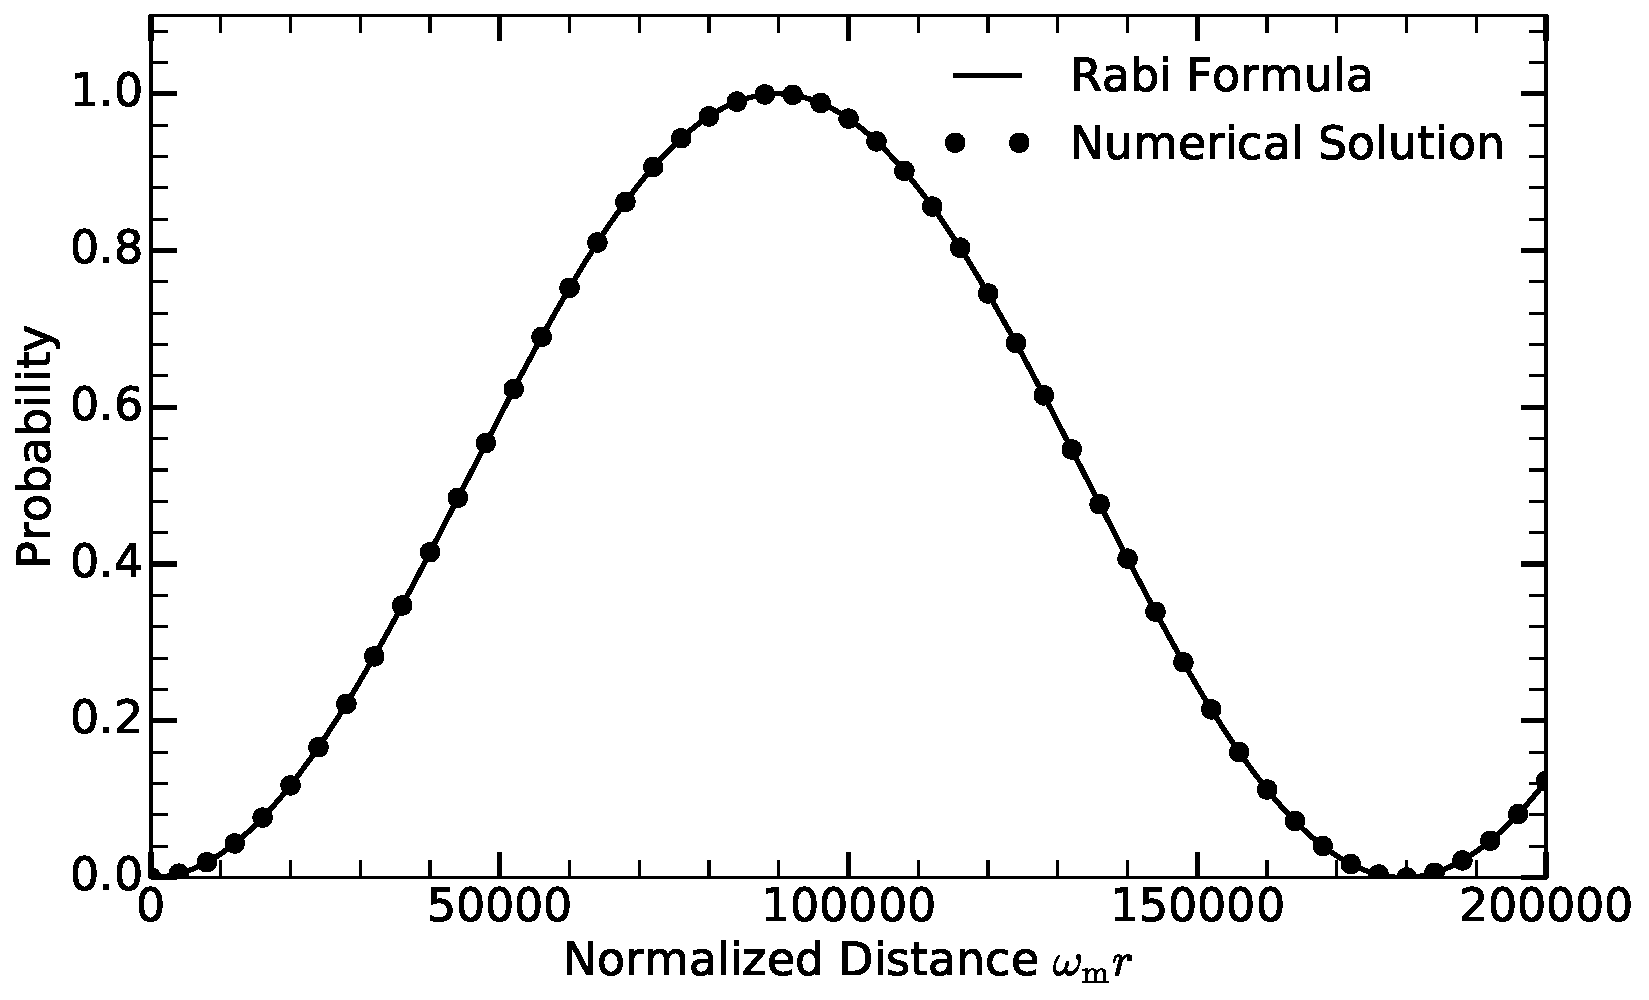
\includegraphics[width=\columnwidth]{assets/rabiOscillationsNeutrinoCoincidence-single-frequency}
                %rabiOscillationsNeutrinoCoincidence}
                \caption{Single frequency matter profile and Rabi oscillation. The markers are numerical results for the transition probabilities between two background mass eigenstates for the neutrinos with matter perturbation $A_1\sin(k_1 r)$. The dots, diamonds, and squares are for $k_1=\omega_{\mathrm m}$, $k_1=(1-2\times 10^{-5})\omega_{\mathrm m}$, and $k_1=(1-10^{-4})\omega_{\mathrm m}$ respectively. The lines are the predictions using Rabi formula. During the calculation, $\lambda_0$ is set to $0.5$ of the MSW resonance potential $\lambda_{\mathrm{MSW}}=\omega_{\mathrm{v}}\cos 2\theta_{\mathrm v}$ and mixing angle is chosen so that $\sin^2(2\theta_{\mathrm v}) = 0.093$.}
                \label{fig-rabiOscillationsNeutrinoCoincidence}
\end{figure}

In FIG.~\ref{fig-rabiOscillationsNeutrinoCoincidence}, we plotted the numerical results using markers as well as the prediction using Rabi formula using lines. The agreement between numerical solutions of neutrino transitions between mass states and Rabi formula will be explained more precisely in Sec.~\ref{sec:jacobi}. For now, we address the significance of relative detuning $\RD = \lvert k_1 - \omega_{\mathrm m} \rvert /\lvert A_1 \rvert$,  which is defined in Appendix~\ref{sec:rabi-oscillations}. It measures how off-resonance a system is. We know that $\RD\to 0$ indicates the system is very close to resonance, while $\RD\to \infty$ indicates the system is far away from resonance. The corresponding relative detunings are $0$, $1.0$, and $5.2$ for $k_1=\omega_{\mathrm{m}}$, $k_1=(1-2\times 10^{-5})\omega_{\mathrm m}$, and $k_1=(1-10^{-4})\omega_{\mathrm m}$.

% 0, 0.516197,1.03239,5.16197

For a single-frequency perturbation in matter profile $\lambda(r) =\lambda_1 +  \lambda_1\sin(k_1 r)$, P. Krastev and A. Smirnov concluded that the parametric resonance condition is $\omega_{\mathrm{m}} \sim n k_1$, if instantaneous $\omega_{\mathrm{m,inst}}(r)$ associated with the matter profile at distance $r$ varies slowly~\cite{Krastev1989}. This condition is exactly the Rabi resonance condition when $n=1$, as such condition matches the driving field frequency to the energy split. Higher order effects are explained in Sec.~\ref{sec:single-revisted}.





\section{\label{sec:multiple}Interference of Rabi Oscillations and Multi-frequency Matter Profile}


The approach applied to single frequency matter profile also helps with the understanding of multi-frequency matter profile. However, multi-frequency matter profile leads to multiple modes of Rabi oscillations, even with our simplified approach by dropping the varying $\sigma_3$ term in Hamiltonian. In this section, we examine the interference between two modes of Rabi oscillations.
%Castle wall matter profile will serve as an example of multi-frequency profile to illustrate the idea of interference.



%%%%%%%%%
%%%% Interference
%%%%%%%%



%\subsection{\label{sec:interference-with-long-wavelength-mode}Interference Between Different Frequencies}

% \fbox{
% \parbox{0.9\columnwidth}{
% \begin{itemize}
%     \item Two limits: strong interference regime and low-interference regime
%     \item For strong interference we include multiple modes
%     \item For weak interference, we can interpret the case that one of the matter profile wavelength is much larger than the other. In this case we have a shift of background matter density of the short wavelength perturbation profile.
%     \item Examples. A slight shift in the background density could remove the resonance, which can be quantified.
%     \begin{equation*}
%         a
%     \end{equation*}
% \end{itemize}
% }
% }


We explain the interference between different modes of Rabi oscillations using the idea of energy gap shift. Suppose we have a Rabi oscillation system with two modes, one mode at resonance with frequency $k_1=\omega_{\mathrm m}$ and another mode with frequency $k_2$ that is off resonance. In some cases, there can be a significant transition amplitude decrease because of the off resonance frequency $k_2$, which can be interpreted as shift of energy gap due to the frequency $k_2$. To model the effect, we construct a Rabi oscillation Hamiltonian with two modes of different frequency,
\begin{widetext}
\begin{equation}
H^{(\mathrm{m})}  = -\frac{\omega_{\mathrm{m}}}{2} \sigma_3 - \frac{1}{2} \sum_{n=1}^N  A_n \cos (k_n r) \sigma_1 + \frac{1}{2} \sum_{n=1}^N  A_n \sin (k_n r) \sigma_2,
\label{eq-hamiltonian-rabi-two-modes-interference}
\end{equation}
\end{widetext}
where $N=2$ for two frequency case. To show the destruction effect, the Hamiltonian Eq.~(\ref{eq-hamiltonian-rabi-two-modes-interference}) is reformed into a vector with sigma matrices $(\sigma_1,\sigma_2,\sigma_3)$ as the basis,
\begin{equation}
\mathbf H = \begin{pmatrix}
0\\
0\\
\omega_m
\end{pmatrix} + \begin{pmatrix}
A_1 \cos (k_1 r)\\
-A_1 \sin (k_1 r)\\
0
\end{pmatrix} + \begin{pmatrix}
A_2 \cos (k_2 r)\\
-A_2 \sin (k_2 r)\\
0
\end{pmatrix}.
\end{equation}

The three terms are defined as $\mathbf  H_3$, $\mathbf H_1$, and $\mathbf H_2$ respectively. $\mathbf H_1$ and $\mathbf H_2$ are two rotating vectors as a function of $r$ with frequencies $k_1$ and $k_2$ in this vector space, while $\mathbf H_3$ is perpendicular to $\mathbf H_1$ and $\mathbf H_2$. To work out the energy gap shift, we go to the frame that corotates with $\mathbf H_2$, in which we have the new frequencies $k_1'=k_1-k_2$ and $k_2'=0$ as well as new energy gap $\omega_{\mathrm m}' = \omega_{\mathrm m}- k_2$. The resonance mode $\mathbf H_1$ retains on the resonance condition since $k_1'=\omega_{\mathrm m}'$, i.e. $k_1-k_2 = \omega_{\mathrm m}-k_2$, holds in the new frame. On the other hand, we have two static fields $\mathbf H_3$ and $\mathbf H_2$ together as the new energy gap, as long as $\mathbf H_2\ll \mathbf H_3$, which is the usual case. The new energy gap in this frame is calculated as
\begin{align}
    \tilde\omega_{\mathrm{m}}' =& \sign (\omega_{\mathrm m}') \sqrt{\omega_{\mathrm{m}}'^2 + A_2^2 } \nonumber\\
    \approx & \omega_{\mathrm{m}}' + \frac{A_2^2}{2\omega_{\mathrm m}'} \nonumber\\
    =& \omega_{\mathrm m} - k_2 + \frac{1}{2}\frac{A_2^2}{\omega_{\mathrm m} - k_2},
    \label{eq-new-energy-gap-due-to-second-mode-approximation}
\end{align}
where we kept only first order of Taylor series. The Taylor expansion in Eq.~(\ref{eq-new-energy-gap-due-to-second-mode-approximation}) holds as long as the relative detuning for the second frequency is large which means the second frequency is off resonance. As an approximation, the transitions between the two energy states follows the Rabi oscillations with energy gap $\tilde \omega_{\mathrm m}'$ and driving field with frequency $k_1'=k_1-k_2$. Consequently, we can estimate how much the amplitude of the transition is suppressed due to $k_1$ mode by calculating the new relative detuning,
\begin{align}
    \RD' =& \frac{\lvert k_1' - \tilde \omega_{\mathrm m}' \rvert}{\lvert A_1 \rvert}\nonumber\\
    =& \left \lvert \frac{ k_1-\omega_{\mathrm m}}{ A_1} + \frac{ A_2^2 }{2  A_1 ( k_2 - \omega_{\mathrm m})} \right  \rvert\\
    =& \left \lvert  \frac{\sign({ k_1-\omega_{\mathrm m}})}{\sign (k_2 - \omega_{\mathrm m})} \RD_1 +  \frac{ A_2 }{2 A_1 \RD_2 }\right \rvert ,
    \label{eq-relative-detuning-changed}
\end{align}
where $\RD_2$ is the relative detuning of the second mode,
\begin{equation*}
\RD_i =  \left\lvert \frac{ k_i - \omega_{\mathrm m}}{A_i} \right \rvert.
\end{equation*}
In principle, you can change the energy gap of the first frequency to approach the resonance or escape the resonance by carefully arranging the second frequency, which is also obvious from Eq.~(\ref{eq-relative-detuning-changed}). However, for the purpose of the paper we only discuss the most important destruction effect by choosing $\RD_1 = 0$. We observe the importance of the relative detuning. For the second mode to significantly interfere with the first mode, we need a small $\RD_2$ and a large amplitude or width $A_2\gg A_1$.

The condition can be verified by comparing the numerical solution and estimation using Rabi formula. However, we are most interested in the amplitude change due to $\mathbf H_2$ mode. Relative detuning is the only variable that we need to calculate the amplitude, hence we only compare the numerical results with estimated amplitudes using $1/(1+\RD'^2)$.
To verify the condition, we choose the first rotating perturbation to satisfy the resonance condition $k_1=\omega_{\mathrm{m}}$, the condition for the second rotating field shifting the system out of resonance is that the relative detuning becomes larger than $1$, which leads to
\begin{equation}
\lvert A_2 \rvert \geq \sqrt{2\omega_{\mathrm{m}} \lvert A_1 (k_2-\omega_{\mathrm m})\rvert} \equiv A_{2,\mathrm{Critical}}.
\end{equation}
We expect the transition amplitude to decrease as we have larger $\lvert A_2\rvert$.


\begin{figure}
                \centering
                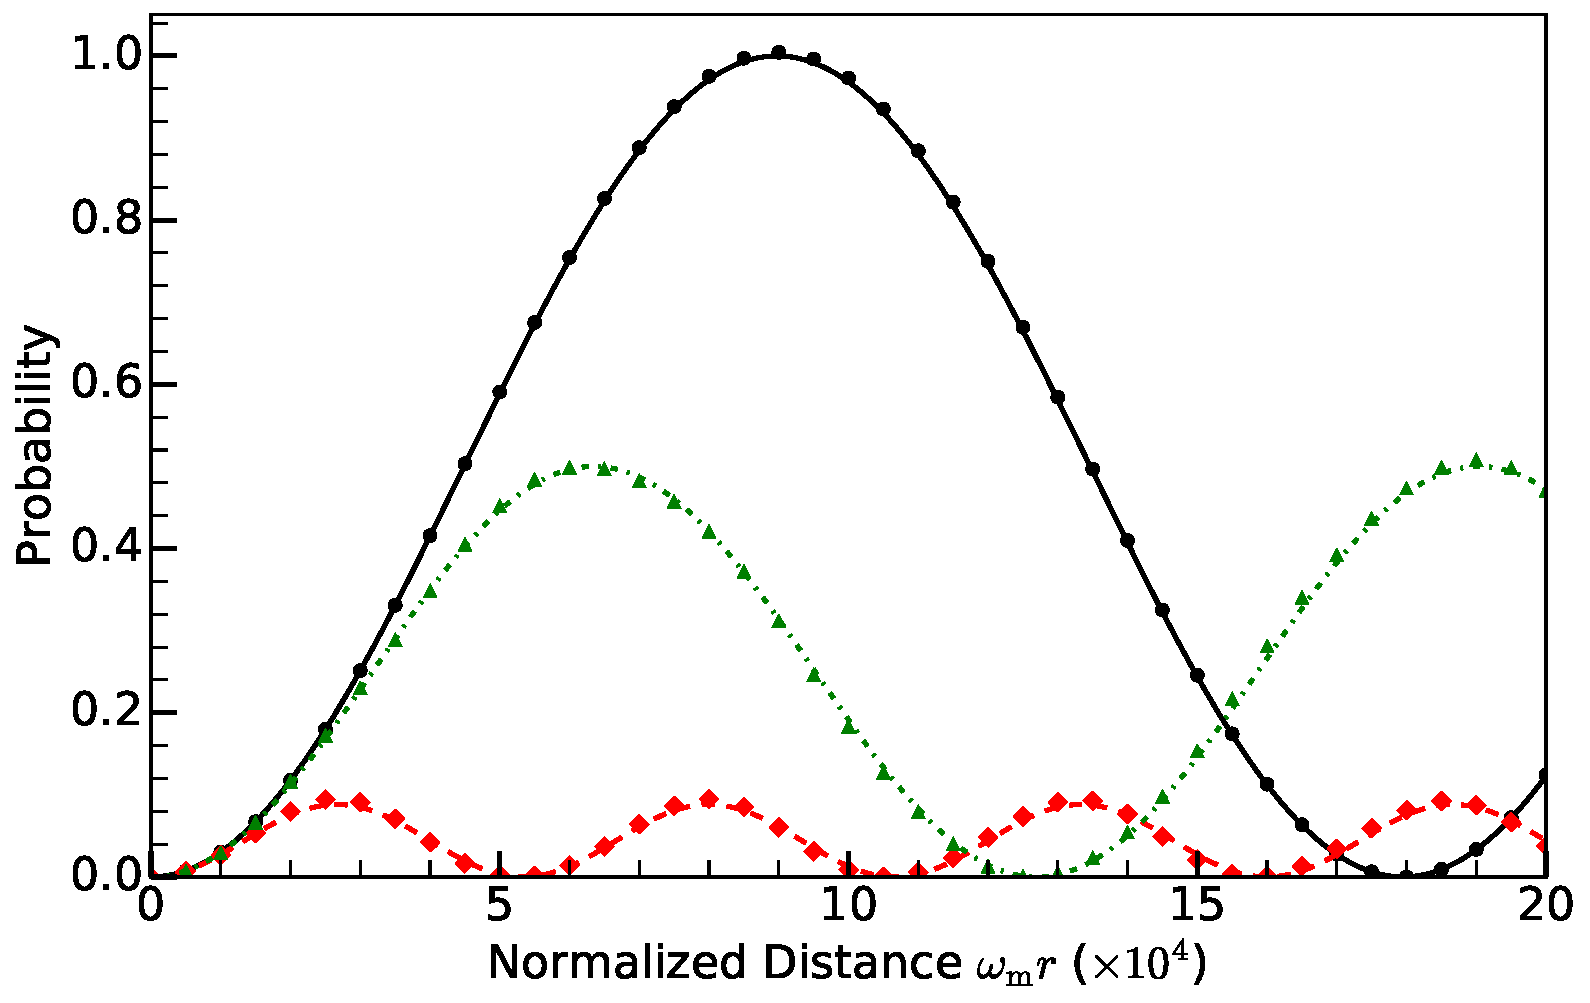
\includegraphics[width=\columnwidth]{assets/interference-reduction}
                \caption{Reduction of transition amplitudes due to interference. Dashed line, dotted line, dash-dotted line, and solid line are for $A_2=10^{-2}\omega_{\mathrm{m}}$, $k_2=10\omega_{\mathrm m}$, $A_2=10^{-2}\omega_{\mathrm{m}}$, $k_2=10^{-1}\omega_{\mathrm m}$, $A_2=5.0\times 10^{-2}\omega_{\mathrm{m}}$, $k_2=10\omega_{\mathrm m}$, and $A_2=5\times 10^{-2}\omega_{\mathrm{m}}$, $k_2=10^{-1}\omega_{\mathrm m}$. In all the calculations, we choose $A_1=10^{-4}\omega_{\mathrm m}$, $k_1=\omega_{\mathrm m}$. The grid lines are the transition amplitudes estimated using $\RD'$. During the calculation, $\Lambda_0$ is set to half of the MSW resonance potential, $\Lambda_0 = \frac{1}{2}\lambda_{\mathrm{MSW}}=\frac{1}{2}\omega_{\mathrm{v}}\cos 2\theta_{\mathrm v}$.}
                \label{fig-rabi-oscillations-energy-gap-change}
\end{figure}


We choose the two modes where the first one has amplitude $A_1 = 10^{-4}\omega_{\mathrm{m}}$ and frequency $k_1 = \omega_{\mathrm{m}}$. With a small amplitude of the second frequency, $A_2=10^{-4}\omega_{\mathrm{m}}$, and large frequency $k_2=10\omega_{\mathrm{m}}$, we obtain almost full resonance. For larger $A_2$ the destruction effect is more effective, as shown in Fig.~\ref{fig-rabi-oscillations-energy-gap-change}. The estimations of transition amplitude are in good agreement with the numerical results. To show the importance of relative detuning, we calculated the relative detuning for each cases, which are $0.06$, $0.6$, $1.4$, $13.9$ for the lines from top to down. We also notice that the width of each cases doesn't change since we kept $A_1$ fixed for each calculation, which indicates that the decreasing in transition amplitude is because of the increasing in detuning.

Even for the single frequency matter profile, there are two modes of Rabi oscillations $\pm k_1$, under the approximation that the varying $\sigma_3$ term in Hamiltonian is neglected, as mentioned in Sec.~\ref{sec:single}. The three examples calculated in Fig.~\ref{fig-rabiOscillationsNeutrinoCoincidence} are almost exact since the modification of relative detuning for the $k_1$ mode that we kept, due to the far off resonance mode $-k_1$ that we neglected, is tiny. The first two lines of Table.~\ref{tab-q-values-single-frequency-example} show the relative detunings of the three cases in Fig.~\ref{fig-rabiOscillationsNeutrinoCoincidence}, where $n=\pm 1$ are for the $\pm k_1$ modes in the Hamiltonian \ref{eq-hamiltonian-bg-matter-basis-single-frequency}. We observe in Fig.~\ref{fig-rabiOscillationsNeutrinoCoincidence} that the relative detuning change due to an extra $-k_1$ mode is not observable.



%%%%%%%%%%%%%%%%%%%%%%%%%%%%%%%%%%%%%%%%%%%%%%%%%%%%
%%%%%%%%%  Stimulated Neutrino Oscillations  %%%%%%%%%%%%%%%%%%%
%%%%%%%%%%%%%%%%%%%%%%%%%%%%%%%%%%%%%%%%%%%%%%%%%%%%

\section{\label{sec:jacobi}Parametric Resonance and Rabi oscillation --- Jacobi-Anger expansion}


With the intuition of the Rabi oscillations itself as well as the interference between different modes of Rabi oscillations shown in Sec.~\ref{sec:multiple}, we expect to interpret the transition probabilities of any matter profile more precisely if the system can be exactly decomposed into multiple Rabi oscillations. Kneller et. al provided a method to achieve this goal~\cite{Kneller2013}, namely the Jacobi-Anger expansion. In this section, we show that the matter effect can be decomposed into superpositions of Rabi oscillations by applying a Jacobi-Anger expansion to the Hamiltonian. Our approach is to apply a designed unitary transformation first which make the motivation of Jacobi-Anger expansion, before writing down the final result as superpositions of Rabi oscillation using Jacobi-Anger expansion. For a system with general matter perturbation, c.f. Eq.~(\ref{eq-hamiltonian-bg-matter-basis-general}), we apply an unitary transformation of the form
\begin{equation}
    \mathbf{U} =  \begin{pmatrix} e^{-\ri \eta (r)} & 0 \\  0 & e^{\mathrm i \eta (r)}  \end{pmatrix},
    \label{eq-rabi-transformation}
\end{equation}
which is a transformation used in Ref.~\onlinecite{Kneller2006} to remove the diagonal elements of the Hamiltonian. This transformation is essentially a rotation $\exp\left(-\mathrm i\frac{\sigma_3}{2}\cdot 2\eta\right)$. In this work, this transformation is used to remove the varying $\sigma_3$ terms $\delta\lambda(r) \cos 2\theta_{\mathrm m} \sigma_3/2$ in the Hamiltonian, so that the energy gap is fixed in the new basis $\left(\ket{\nu_{\mathrm{r1}}},\ket{\nu_{\mathrm{r2}}}\right)^{\mathrm{T}}$, which is defined as
\begin{equation}
    \begin{pmatrix} \ket{\nu_{\mathrm{r1}}}\\ \ket{\nu_{\mathrm{r2}}} \end{pmatrix} =  \mathbf{U}^\dagger \begin{pmatrix} \ket{\nu_{\mathrm{L}}} \\ \ket{\nu_{\mathrm{H}}} \end{pmatrix}.
    \label{eq-rabi-basis}
\end{equation}
For convenience, we name this unitary transformation in Eq.~(\ref{eq-rabi-transformation}) Rabi transformation as well as the new basis in Eq.~(\ref{eq-rabi-basis}) the Rabi basis. The reason it can remove the $\sigma_3$ term is that it will transform the system into a rotating frame so that the varying energy gap due to the fluctuating matter density is exactly cancelled by rotation of the frame. In Rabi basis, we find the Schr\"{o}dinger equation
\begin{widetext}
\begin{equation*}
    \begin{pmatrix}  \frac{\mathrm d\eta}{\mathrm dr}  & 0 \\ 0 & - \frac{\mathrm d\eta}{\mathrm d r}  \end{pmatrix} \begin{pmatrix} \psi_{\mathrm R1} \\ \psi_{\mathrm R2} \end{pmatrix} + \mathrm i \frac{\mathrm d}{\mathrm dr} \begin{pmatrix} \psi_{\mathrm R1} \\ \psi_{\mathrm R2} \end{pmatrix}
    = \left[ -\frac{\omega_{\mathrm m} }{2} \sigma_3  + \frac{\delta \lambda}{2} \cos 2\theta_{\mathrm m}  \sigma_3  - \frac{\delta \lambda}{2} \sin 2\theta_{\mathrm m} \begin{pmatrix} 0 & e^{2\mathrm i\eta} \\ e^{-2 \mathrm i\eta } & 0 \end{pmatrix}   \right] \begin{pmatrix} \psi_{\mathrm R1} \\ \psi_{\mathrm R2} \end{pmatrix},
\end{equation*}
\end{widetext}
in which the varying diagonal elements in Hamiltonian can be eliminated by choosing $\eta(r)$ properly, i.e.,
\begin{equation}
    \eta(r) - \eta(0) =  \frac{\cos 2\theta_{\mathrm{m}}}{2} \int_0^r \delta\lambda (\tau) d\tau.
\end{equation}
In Rabi basis, the Schr\"{o}dinger equation becomes
%\begin{widetext}
\begin{equation*}
    \ri \frac{d}{dr} \begin{pmatrix} \psi_{\mathrm r1} \\ \psi_{\mathrm r2} \end{pmatrix} = \left[ - \frac{\omega_{\mathrm m}}{2} \sigma_3 - \frac{\delta \lambda}{2} \sin 2\theta_{\mathrm m} \begin{pmatrix} 0 & e^{2\ri\eta} \\ e^{-2 \ri \eta } & 0 \end{pmatrix}\right] \begin{pmatrix} \psi_{\mathrm r1} \\ \psi_{\mathrm r2} \end{pmatrix}.
\end{equation*}
%\end{widetext}
One can easily show that the transition probability between two eigenstates in Rabi basis is the same as the transition probability between two eigenstates in background matter basis, given the initial condition that the system is in low energy state.

For single frequency matter profile with potential $\delta\lambda(r) = A_1\sin(k_1 r)$, we have $\eta(r) = - A_1 \cos 2\theta_{\mathrm m} \cos (k_1 r)/(2 k) $. To make connection with Rabi oscillation, we apply Jacobi-Anger expansion, which is used in Ref.~\onlinecite{Kneller2013}, to decompose the $\exp\left( \ri z \cos\left(k_1 r \right) \right)$-like term in Hamiltonian into linear combinations of terms that is proportional to $\exp\left(\ri n k_1 r \right)$, i.e., to decompose spherical waves into plane waves. The decomposed form of Hamiltonian explicitly shows that the Hamiltonian is a summation of Rabi systems, which is
%\begin{widetext}
\begin{equation*}
    H^{(\mathrm{R})} =
    -\frac{\omega_{\mathrm{m}}}{2} \sigma_3
    -  \frac{1}{2} \sum_{n=-\infty}^\infty B_n \begin{pmatrix}
    0 &  \Phi_n e^{\ri n k_1  r} \\
     \Phi_n^* e^{ - \ri n k_1 r} & 0
    \end{pmatrix},
\end{equation*}
%\end{widetext}
where
\begin{align*}
    B_n &= \tan 2\theta_{\mathrm m} n k_1 J_{n} \left( \frac{A_1}{k_1}\cos 2\theta_{\mathrm m} \right),\\
    \Phi_n &= e^{i\pi (3n/2+1)},
\end{align*}
with $J_n$ standing for the Bessel function.
The constant phase $\Phi_n$ doesn't play any role for the reason discussed in Appendix~\ref{sec:rabi-oscillations}. Phase in matter potential would also go into $\Phi_n$, for which reason, phase of matter profile is not included in the current discussion. In the Hamiltonian, the first term describes the energy gap, while the second term is the summation of many driving fields. The resonance width for a given mode $n$ is $\lvert B_{n}\rvert$. It's worth mentioning that we have~\cite{Ploumistakis20092897}
\begin{equation}
J_n(n \sech \alpha) \sim \frac{ e^{n(\tanh\alpha - \alpha)} }{\sqrt{ 2\pi n \tanh \alpha } }
\end{equation}
for large $n$. It's straightforward to prove that resonance width decreases dramatically for large $n$ thus resonance of higher order modes become insignificant.



When the system has one dominate resonance mode and without significant interference between the resonance mode and other modes, all off-resonance modes can be dropped without significantly changing the transition probabilities. However, as we have shown previously in Sec.~\ref{sec:multiple}, interference might happen between different modes and interferences were measured with a criteria. However, interference is not the only effect we need to consider. The following subsections will determine the important modes of the system (i.e., which $n$ to include) and explore the interference between modes hence explain the coincidence presented in the previous sections. We use dimensionless quantities which are scaled using the characteristic energy scale $\omega_{\mathrm{m}}$, e.g.,
\begin{align*}
    \hat r &= \omega_{\mathrm{m}}r, \\
    \hat k_1 & = \frac{k_1}{\omega_{\mathrm{m}}}, \\
    \hat A_1 & = \frac{A_1}{\omega_{\mathrm{m}}}, \\
    \hat B_n &= \frac{B_n}{\omega_{\mathrm{m}}}.
\end{align*}

%Through the Rabi transformation and Jacobi-Anger expansion, the varying diagonal elements in Hamiltonian, i.e., varying $\sigma_3$ term, is transformed to a perturbing field with many different frequencies $n k_1$.






\subsection{The Important Factors}


In order for a mode to have a significant effect on the transition probabilities, we require it to has large relative detuning $\RD$, and a large oscillation wavelength compared to the size of the physical system. Relative detuning for each mode is calculated as
\begin{equation}
\RD_n = \frac{\lvert n k_1 - \omega_{\mathrm{m}} \rvert}{B_n}
\end{equation}
for single frequency matter profile, and
\begin{equation}
\RD_{\{n_a\}} = \frac{\lvert \sum_a n_a k_a -\omega_{\mathrm m} \rvert }{B_{\{n_a\}}}
\end{equation}
for multi-frequency matter profile.


For modes with small relative detuning, they are important since they might lead to full transition. However, the full transition requires at least a distance of the order of the wavelength of the oscillation. Suppose we have a mode that has zero relative detuning, but with a oscillation wavelength much larger than the size of the system, such a mode would never have the chance to accumulate a large transition probability within the size of the system. By utilizing the theory of Rabi oscillation, we know that the oscillation wavelength of each mode is determined by the Rabi frequency
\begin{equation}
\Omega_{\{n_a\}} = \lvert B_{\{n_a\}} \rvert \sqrt{1+\RD_{\{n_a\}}^2}.
\end{equation}
Thus modes that has much larger oscillation wavelength are not subjected to be considered even though their relative detunings are close to zero.

In principle, we can always approximate the system by including more modes with larger relative detuning while neglecting the modes with wavelength much longer than the size of physical system. However such effort doesn't simplify the calculations.




\subsection{\label{sec:single-revisted}Single Frequency Matter Profile Revisited}

For the single frequency matter potential $\lambda = \lambda_0 + \lambda_1 \sin(k_1 r)$ discussed in Sec.~\ref{sec:single}, we removed the varying $\sigma_3$ term by arguing that this term has no effect on transition probabilities when the system is close to resonance, $k_1 \sim \omega_{\mathrm m}$. The reason is that only the first mode $n=1$ is on resonance when $k_1=\omega_{\mathrm m}$ and all other modes are far from resonance, thus
\begin{align}
H^{\mathrm R} \approx & -\frac{\omega_{\mathrm m}}{2}\sigma_3 - \frac{1}{2} B_1 \begin{pmatrix}
0 & \Phi_1 e^{i k_1 r} \\
\Phi_1^* e^{-ik_1r} & 0
\end{pmatrix}\label{eq-single-frequency-first-mode-hamiltonian} \\
\approx & -\frac{\omega_{\mathrm m}}{2} \sigma_3 - \frac{A_1}{2} \cos(k_1 r) \sigma_1 + \frac{A_1}{2} \sin(k_1 r) \sigma_2\nonumber,
\end{align}
where $A_1$ is defined in Eq.~(\ref{eq-define-a1}) and approximation
\begin{equation*}
J_1\left( \frac{\lambda_1}{k_1}\cos (2\theta_{\mathrm m}) \right) \approx \frac{\lambda_1}{2k_1}\cos (2\theta_{\mathrm m})
\end{equation*}
for $\lambda_1\cos(2\theta_{\mathrm m})/k_1\ll 1$ is used in the last step. Thus we reach a similar equation to the approximation we used in Sec.~\ref{sec:single}. $\lambda_1\cos(2\theta_{\mathrm m})/k_1\ll 1$ corresponds to small resonance width for Eq.~(\ref{eq-hamiltonian-bg-matter-basis-single-frequency}) and also Eq.~(\ref{eq-single-frequency-first-mode-hamiltonian}) so that the interferences are small.


Using Jacobi-Anger expansion, we can calculate the relative detuning for each mode as well as the interference effect. The relative detuning for each mode in the Jacobi-Anger expansion for single frequency matter profile used in Fig.~\ref{fig-rabiOscillationsNeutrinoCoincidence} is calculated and listed in Table.~\ref{tab-q-values-single-frequency-example}. The $\RD'_1$ is the shifted relative detuning of the first mode with $n=1$ due to other mode. It clearly shows that the first mode takes the whole system so that the approximation of neglecting the varying $\sigma_3$ terms in Hamiltonian is accurate enough. One can also show that the interference effect due to higher order modes is negligible, since they do not change the relative detuning of the most significant modes.



% {
%  {{1}, 0.},
%  {{-1}, 103239.},
%  {{2}, 1.11987*10^9},
%  {{-2}, 3.3596*10^9},
%  {{3}, 9.71798*10^13},
%  {{-3}, 1.9436*10^14},
%  {{4}, 9.48722*10^18}
% }
% {324336., 3.14159, 6.28319, 2.0944}

% {
%  {{1}, 1.03239},
%  {{-1}, 103238.},
%  {{2}, 1.1198*10^9},
%  {{-2}, 3.35948*10^9}
% }
% {225656., 3.14162, 6.28356, 2.09446}

% {
%  {{1}, 5.16197},
%  {{-1}, 103234.},
%  {{2}, 1.11953*10^9},
%  {{-2}, 3.35904*10^9}
% }
% {61685., 3.14175, 6.28507, 2.09474}

\begin{table*}
\caption{\label{tab-q-values-single-frequency-example}Relative detuning and oscillation wavelength of each mode for single frequency matter profile.}
\begin{ruledtabular}
\begin{tabular}{llll|llll|llll}
 \multicolumn{4}{c|}{$k_1=\omega_{\mathrm m}$} & \multicolumn{4}{c|}{$k_1=(1-2\times 10^{-5})\omega_{\mathrm{m}}$} & \multicolumn{4}{c}{$k_1=(1-10^{-4})\omega_{\mathrm m}$} \\
\hline
   $n$ & $\RD$ & $\RD'_1$  & $2\pi\omega_{\mathrm m}/\Omega_n$ & $n$ & $\RD$ & $\RD'_1$ & $2\pi\omega_{\mathrm m}/\Omega_n$ & $n$ & $\RD$ & $\RD'_1$ & $2\pi\omega_{\mathrm m}/\Omega_n$  \\
\hline
 1 &	0  & - &   $3.2\times10^5$   & 1 &	1 &  -  &   $2.2\times 10^5$       & 1   &	$5.2$ &  - & $6.2\times10^4$   \\
-1 &	$10^5$ &  $4.8\times 10^{-6}$  &   $3.1$     &     -1 &	$10^5$ &   1  &   $3.1$               &  -1 &	$10^5$  & $5.2$ & $3.1$  \\
2 &	$1.1\times 10^9$  &   $2.1\times 10^{-14}$  &   $6.3$    &  2 & 	$1.1\times 10^9$ &  1  &    $6.3$   &  2  &	$1.1\times 10^9$  &  $5.2$  & $6.3$  \\
-2 &	$3.4\times 10^9$  & $6.9\times 10^{-15}$ & $2.1$ &    -2 &	$3.4\times10^9$ &  1  &  $2.1$          & -2  &	$3.4\times 10^9$ & $5.2$ &  $2.1$  \\
\end{tabular}
\end{ruledtabular}
\end{table*}









\subsection{Castle Wall Matter Profile}



For completeness of this paper, we show one example of multi-frequency matter profile. One of the multi-frequency matter profiles that has been well studied is the castle wall matter profile. Using Fourier series, any matter profile can be Fourier decomposed into superposition of many single frequency matter profile in principle. We decompose the periodic castle wall matter profile into many frequencies and study the interference effect. The potential shown in Fig.~\ref{fig-castlewall-profile-illustration} is defined as,
\begin{equation}
    \lambda(r) = \begin{cases}
\Lambda_1, &\quad -\frac{X_1}{2}+nX\le r\le \frac{X_1}{2}+nX \\
\Lambda_2, &\quad \frac{X_1}{2}+nX\le r\le \frac{X_1}{2}+\frac{X_2}{2} +nX
\end{cases}
\label{eq-castle-wall-potential}
\end{equation}
where $X_1$ and $X_2$ are the two periods of the matter profile or potential, $X=X_1+X_2$, and $n$ is integer. The parametric resonance condition derived by E. Akhmedov~\cite{Akhmedov2000} is,
\begin{equation}
    \frac{\tan (\omega_{\mathrm m1}X_1/2)}{\tan (\omega_{\mathrm m2}X_2/2)} = - \frac{\cos 2\theta_{\mathrm m2}}{\cos 2\theta_{\mathrm m1}},
    \label{eq-akhmedov-resonance-condition-castle-wall}
\end{equation}
where $\omega_{\mathrm{m}i}$ and $\theta_{\mathrm{m}i}$ are the energy difference and mixing angle for potential $\Lambda_1$ and $\Lambda_2$ respectively.



Even though this castle wall problem is analytically solved, the resonance condition Eq.~(\ref{eq-akhmedov-resonance-condition-castle-wall}) itself is not transparent. In this subsection, we show that such a system is closed related to Rabi oscillations. For illustration purpose, we set the profile to be equal period for the two densities so that $X_1=X_2\equiv X/2$. To show that the neutrino flavor conversions in this castle wall matter profiles is related to Rabi oscillation, we decompose the profile using Fourier series,
\begin{equation}
\lambda(r) = \lambda_0 + \sum_{n=1}^{\infty} \lambda_n \cos\left( k_n  r \right),
\label{eq-castle-wall-fourier-expanded}
\end{equation}
where
\begin{align*}
\lambda_0 &= (\Lambda_1 + \Lambda_2)/2, \\
\lambda_n & = \frac{2}{(2n-1)\pi}  (-1)^n  \left( \Lambda_1 -  \Lambda_2 \right),\\
k_n &= (2n-1)k_0, \\
k_0 &= 2\pi/X.
\end{align*}

To calculate the transitions between two mass states of background matter potential $\lambda_0$, we use the background matter basis with respect to $\lambda_0$, in which the transition is zero when varying matter profile vanishes. The Hamiltonian
\begin{widetext}
\begin{equation}
H^{(\mathrm m)} = - \frac{1}{2}\omega_{\mathrm m} \sigma_3  + \frac{1}{2} \sum_{n=1}^{\infty} \lambda_n \cos 2\theta_{\mathrm m} \cos\left( k_n  r \right)  \sigma_3 - \frac{1}{2} \sum_{n=1}^{\infty} \lambda_n \sin 2\theta_{\mathrm m}  \cos\left( k_n r \right) \sigma_1,
\label{castle-wall-decomposed-hamiltonian}
\end{equation}
\end{widetext}
determines the transitions between the two background matter states.


\begin{figure}
    \centering
    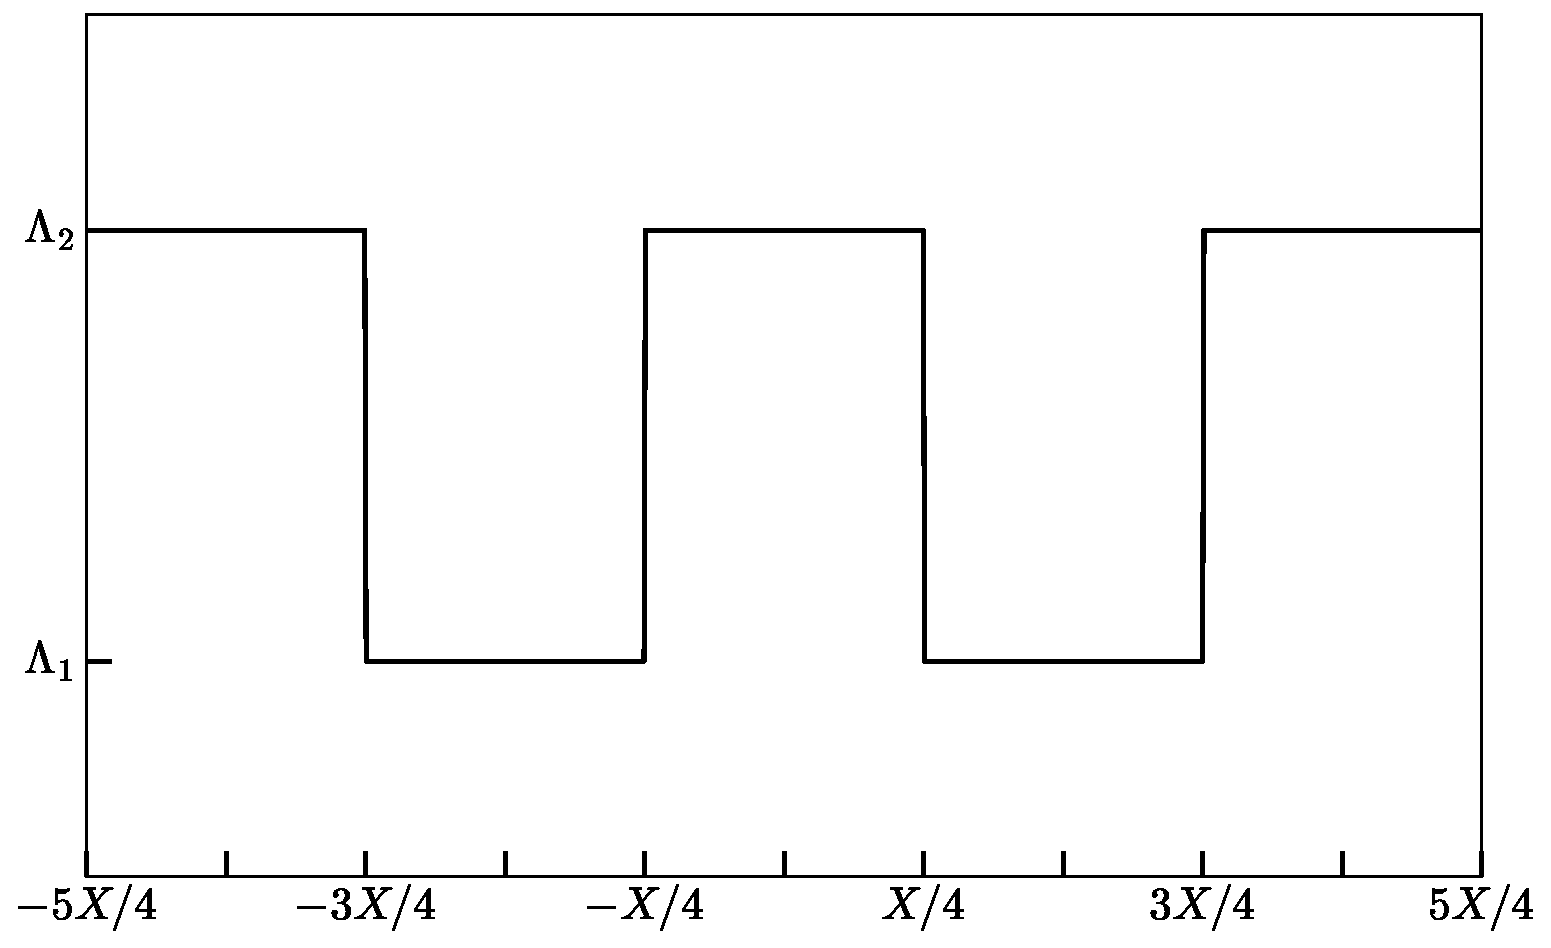
\includegraphics[width=\columnwidth]{assets/castlewall-profile}
    \caption{The castle wall matter potential profile with $X_1=X_2=X/2$.}
    \label{fig-castlewall-profile-illustration}
\end{figure}

\begin{figure}
        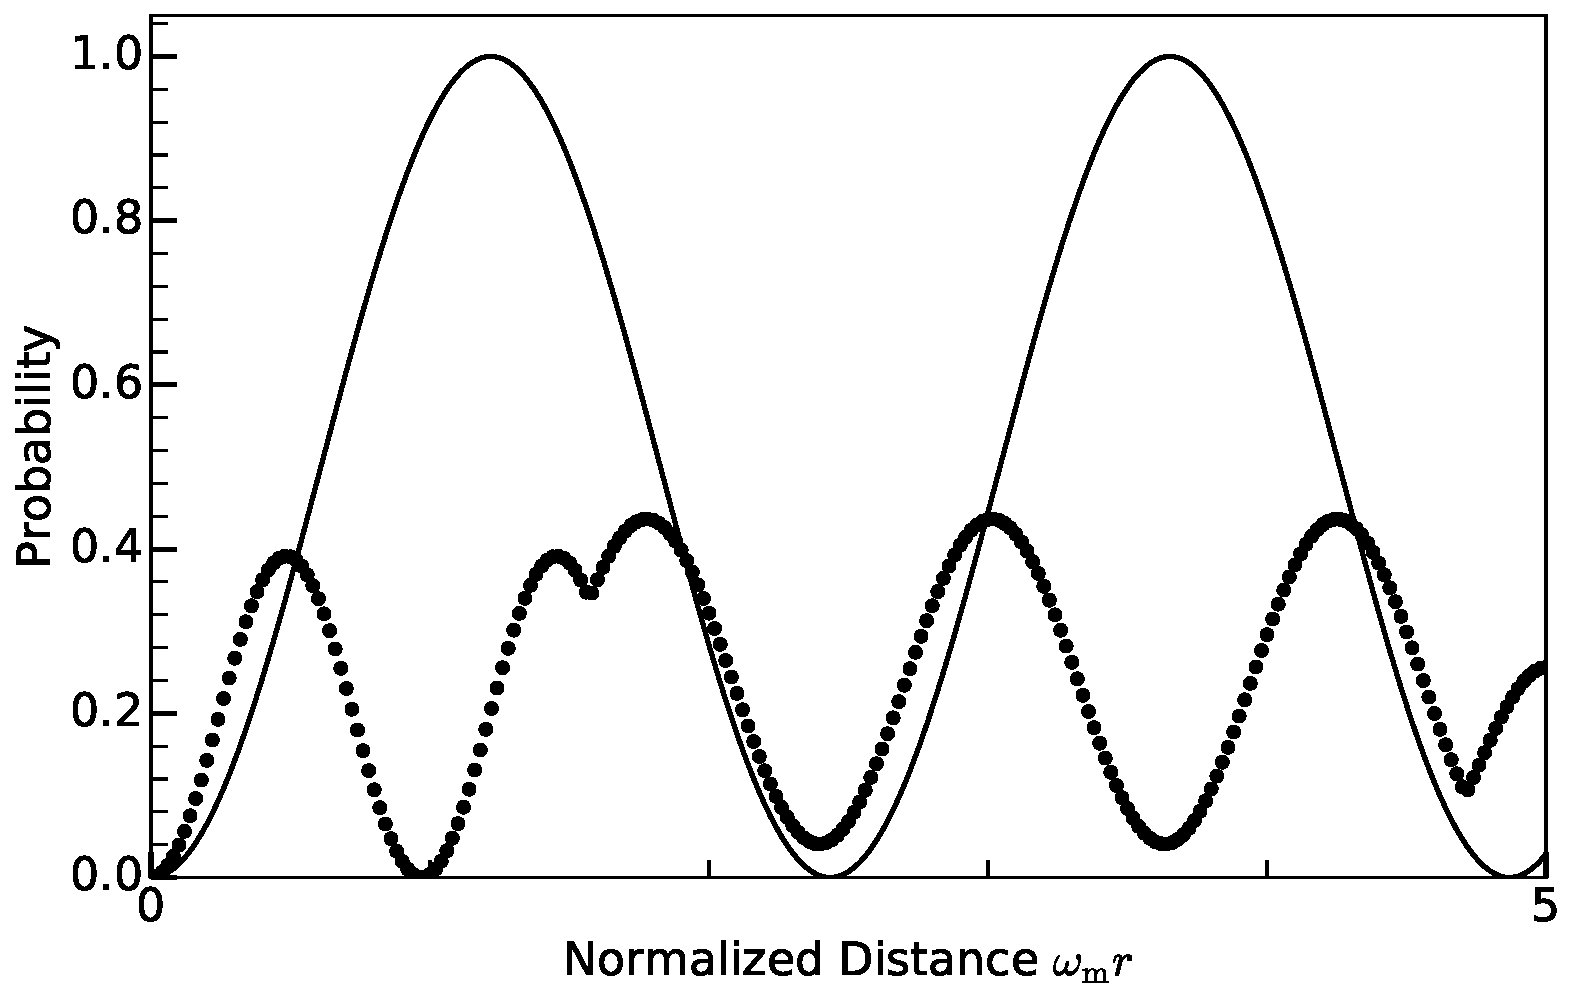
\includegraphics[width=\columnwidth]{assets/castle-wall-1}%
    \caption{Transition probabilities for castle wall matter profile calculated numerically for $\Lambda_2-\Lambda_1=0.4 \Lambda_0$. During the calculation, the energy of neutrinos is $10\,\mathrm{MeV}$, mass-squared difference is $\delta m^2=2.6\times 10^{-3}\,\mathrm{eV^2}$, and the vacuum mixing angle chosen so that $\sin^2(2\theta_v)=0.093$. The background potential $\Lambda_0$ is chosen so that it's half the MSW resonance potential, $\Lambda_0 = \frac{1}{2}\lambda_{\mathrm{MSW}}=\frac{1}{2}\omega_{\mathrm{v}}\cos 2\theta_{\mathrm v}$, and the base frequency is set to $k_0 = 2\pi/X = \omega_{\mathrm{m}}$.
                 }
    \label{fig-akhmedovOscPlt}
\end{figure}
%\end{widetext}


In principle, the base frequency $k_0$ which is determined by the total period $X$ can be arbitrary. In this example, we choose a $X$ so that the base frequency $k_0$ matches the energy gap $\omega_{\mathrm{m}}$. Even though multiple perturbation frequencies show up in Eq.~(\ref{castle-wall-decomposed-hamiltonian}), we identify that only the first frequency $n=1$ is the resonance frequency since we are using $k_0=\omega_{\mathrm{m}}$. As an approximation, we drop all other frequencies $n>2$ regarding the fact that they are far from resonance. Thus, similar to single frequency matter profile, the varying $\sigma_3$ terms have limited effects on the transition probabilities in our case, which leads to
\begin{align*}
    H^{(\mathrm m)} \to & - \frac{1}{2}\omega_{\mathrm m} \sigma_3  - \frac{1}{2} \sum_{n=1}^2\lambda_n \sin 2\theta_{\mathrm m}  \cos\left( k_n r \right) \sigma_1\\
    \to & - \frac{1}{2}\omega_{\mathrm m} \sigma_3  - \frac{1}{2} \sum_{n=1}^2 A_n \cos ( k_n r) \sigma_1 \\
    & + \frac{1}{2} \sum_{n=1}^2A_n \sin(k_n r) \sigma_2,
\end{align*}
where
\begin{equation*}
A_n = \frac{\lambda_n \sin 2\theta_{\mathrm m} }{2} .
\end{equation*}
The relative detuning is $0$ if we have only the first mode. However, it becomes
\begin{equation}
\RD_1'= \frac{A_2^2}{2\lvert A_1 (\omega_{\mathrm m} - k_2) \rvert},
\end{equation}
if we include the second frequency $k_2$. One feature of this Fourier series expanded matter profile Eq.~(\ref{eq-castle-wall-fourier-expanded}) is that the width of each frequency decreases as the order $n$ increases while the detuning of each frequency increases. We calculate the relative detuning for each frequency
\begin{equation}
\RD_n = \frac{\lvert k_n -\omega_{\mathrm m} \rvert}{ \lvert \lambda_n  \sin 2\theta_{\mathrm m}/2 \rvert } = \frac{2(n-1)(2n-1)\pi \omega_{\mathrm m}}{(\Lambda_2 - \Lambda_1)\sin 2\theta_{\mathrm m}}
\end{equation}
which is quadratic in $n$ and inversely proportional to $\Lambda_2-\Lambda_1$. We find that all higher frequencies $k_n$ for $n>2$ have very large relative detunings. The neutrino transition probability between the two matter states is shown in FIG.~\ref{fig-akhmedovOscPlt}, where we find the system has almost full transition.

A more rigorous treatment is to use Jacobi-Anger expansion and find the Rabi modes, where we find that the mode that corresponds to single frequency $k_1$ dominates and all other modes have little destruction effect on it. Quantitatively, higher orders leads to smaller width $B_{\{n_i\}}$ yet larger detuning $\sum_{n} nk_n-\omega_{\mathrm m}$, which renders a smaller effect on the resonance mode $\{1,0\}$, since the effect is evaluated as Eq.~(\ref{eq-relative-detuning-changed}).
Table~\ref{tab-q-values-each-mode} lists the first few smallest relative detunings of Fig.~\ref{fig-akhmedovOscPlt}. The second column is the relative detuning of the corresponding mode, while the third column is the relative detuning of mode $\{1,0\}$ with the energy gap shift effect of the corresponding mode.



% Find the data in MMA file `akhmedov-parametric-resonance.nb`
% {0., 6129.81, 20432.7, 42908.7}
% {0., 5.99981, 19.9994, 41.9987}

\begin{table}
\caption{\label{tab-q-values-each-mode}Relative detuning of each frequency.}
\begin{ruledtabular}
\begin{tabular}{lll}
 $\{n_1,n_2\}$ &  $\RD$ & $\RD'_{\{1,0\}}$   \\
\hline \\
 $\{1,0\}$ & $0$ &  - \\
 $\{-1,0\}$ & $48$ &  $1.0\times 10^{-2}$ \\
 $\{0,1\}$ & $1.5\times 10^2$ &  $1.1\times 10^{-3}$  \\
 $\{2,0\}$ & $2.4\times 10^{2}$ & $2.0\times 10^{-4}$
\end{tabular}
\end{ruledtabular}
\end{table}





\section{\label{conclusions}Conclusions}

%%%% Do not repeat what has been said


In conclusion, we have provided an interpretation for neutrino flavor conversion in fluctuating matter with the help of Rabi oscillations. The work provided two different points of view that is related to Rabi oscillations.

The first point of view was to interpret the neutrino flavor conversions in background matter basis. In this basis, matter density fluctuations will introduced a fluctuation part to the diagonal elements of the Hamiltonian, which means that the energy gap is fluctuating if we draw analogy between this Hamiltonian and the Hamiltonian of Rabi oscillations. For neutrino flavor conversions in a single frequency matter profile, the neutrino flavor oscillations becomes large when the matter fluctuation frequency is close to the energy gap, which is the resonance condition. We anticipated that the fluctuations of energy gap have limited effects on neutrino flavor conversions under this resonance condition. Thus the matter fluctuation only works as a pure flipping field that converts neutrinos from one flavor to another.

As we added more frequencies of matter density fluctuations, the neutrino flavor conversions becomes nontrivial due to the interferences between the difference matter profile frequencies. To quantify the interference between different Rabi oscillation modes, we defined relative detuning which describes how off-resonance a Rabi oscillation is. In the case of single frequency Rabi oscillations, the relative detuning becomes $0$ under the resonance condition. As a second frequency is added to the oscillations, the energy gap is shifted due to this new frequency. A measure of the interference effect is to consider the relative detuning of the first frequency which is at resonance, under the shifted energy gap. Numerical results verified this conjecture. With the interference mechanism, we revisit the single frequency matter profile neutrino oscillations.

Another view is to switch to a basis where the neutrino oscillations Hamiltonian is decomposed into infinite Rabi oscillations. Equivalently speaking, the oscillations are consequences of superposition of Rabi oscillations, which we call modes of oscillations. This view was applied to emphasis the approximations that the change of energy gap due to matter fluctuation can be neglected under resonance condition in the previous background matter basis.











\section{\label{acknowledgement}Acknowledgement}

The first author would like to thank J. Kneller and K. Patton for their help during this research. This research is supported by DOE EPSCoR grant \#DE-SC0008142.




%%%%%%%%%%%%%%%%%%%%%%%%%%%%%%%%%%%%%%%%%%
%%%%%%%%%%%%% APPENDIX  %%%%%%%%%%%%%%%%%%
%%%%%%%%%%%%%%%%%%%%%%%%%%%%%%%%%%%%%%%%%%



% \newpage\null\thispagestyle{empty}
% \vspace{20em}
% This page is intentionally left blank
% \newpage


% \clearpage
\appendix
% \section{\label{sec:three-bases}Three Bases}

% \fbox{Define the three different bases used.}

\section{\label{sec:rabi-oscillations}Rabi Oscillations}

%  trim={<left> <lower> <right> <upper>}
%\begin{widetext}
% \begin{figure*}
%     \centering
%     \begin{subfigure}[b]{0.5\textwidth}
%         \centering
%         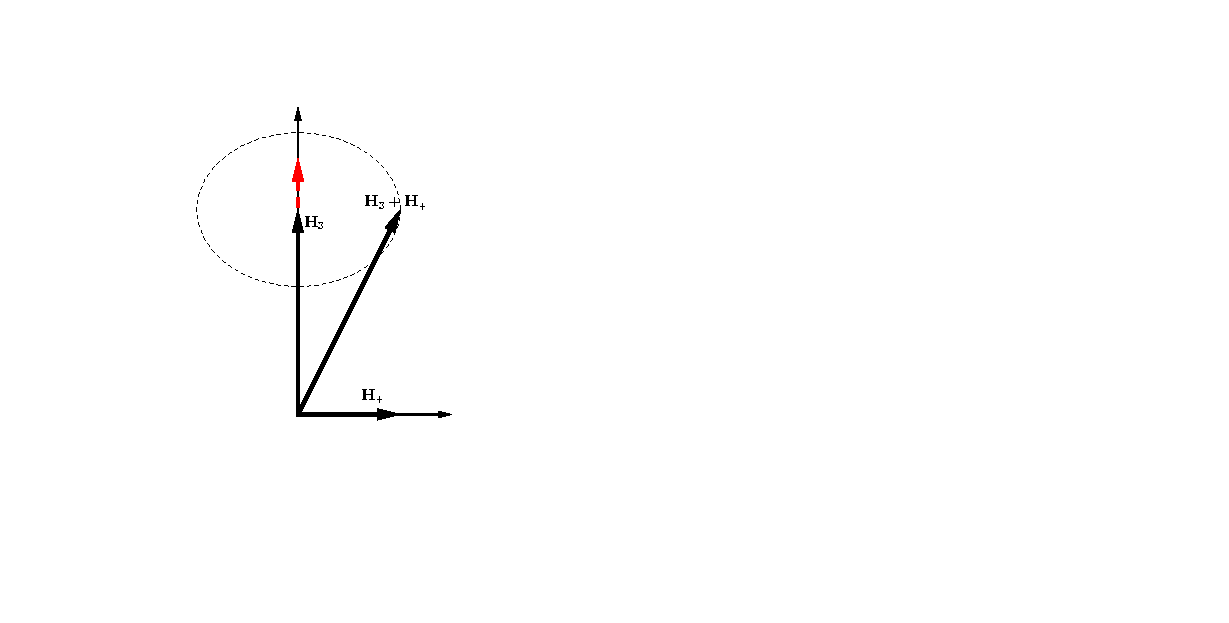
\includegraphics[trim={2cm 3.2cm 9.5cm 1cm},clip]{assets/rabi-isospin-static-frame}
%     \caption{}
%     \label{fig-rabi-isospin-static-frame}
%     \end{subfigure}%
%     ~
%     \begin{subfigure}[b]{0.5\textwidth}
%         \centering
%         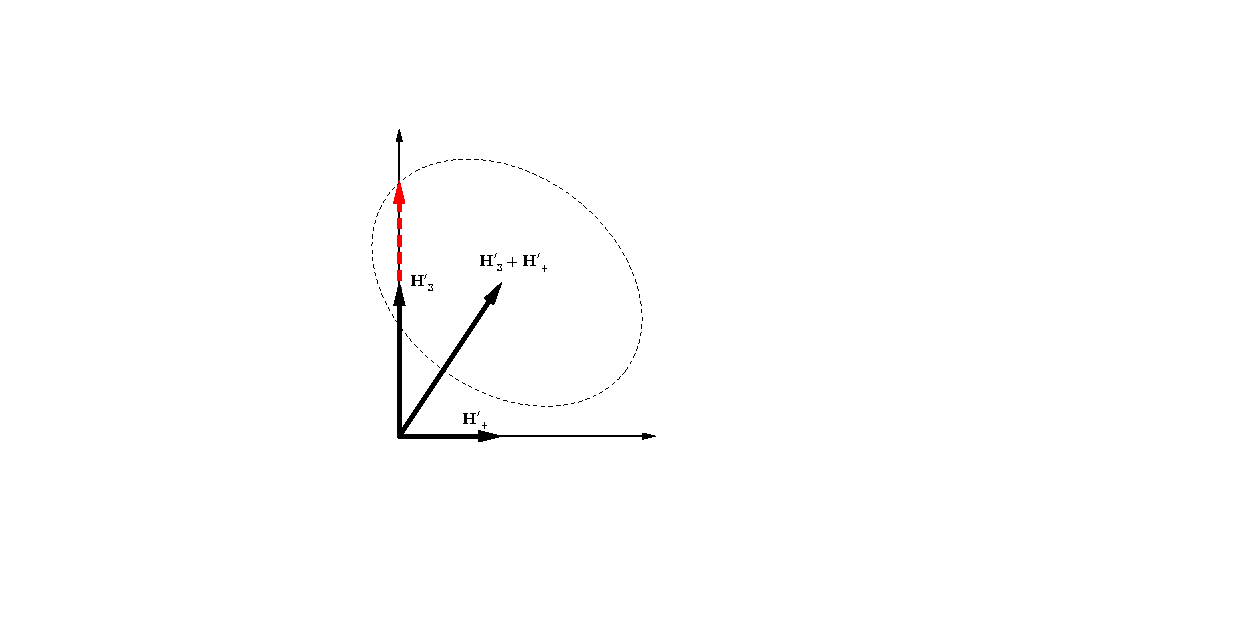
\includegraphics[trim={6cm 3cm 9.5cm 2cm},clip]{assets/rabi-isospin-rotating-frame}
%         \caption{}
%         \label{fig-rabi-isospin-rotating-frame}
%     \end{subfigure}
%     \caption{Rabi oscillations in static frame and rotating frame. In both figures the red dashed vector is the flavor isospin, while the black solid vectors are the vectors of Hamiltonian. The left panel shows the rotating Hamiltonian $\mathbf{H}_3+\mathbf{H}_+$. The right panel shows the rotation of flavor isospin around a static vector $\mathbf{H}'_3+\mathbf{H}'_+$ in the rotating frame.}
%     \label{fig-rabi-isospin-different-frame}
% \end{figure*}
%\end{widetext}

\begin{figure}
        \centering
        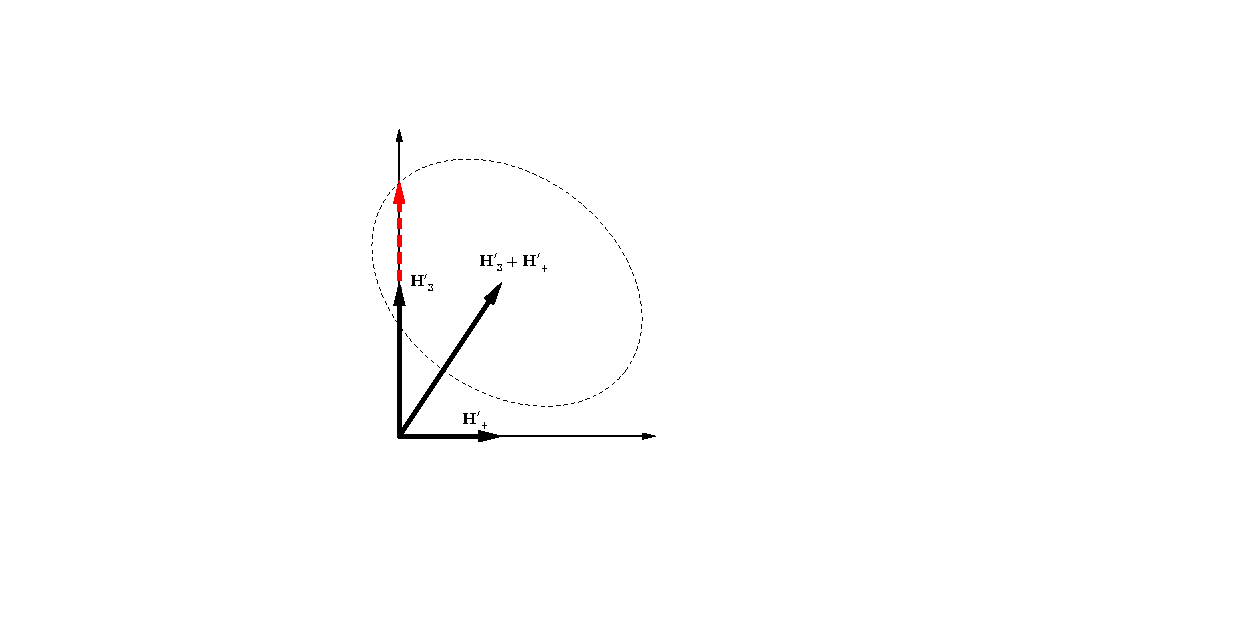
\includegraphics[width=\columnwidth, trim={20cm 10cm 50cm 10cm},clip]{assets/rabi-isospin-rotating-frame}
    \caption{Rabi oscillations in corotating frame. The red dashed vector is the flavor isospin, while the black solid vectors are the vectors of Hamiltonian. The flavor isospin vector is precessing around vector of total Hamiltonian $\mathbf{H}_3+\mathbf{H}_+$.}
    \label{fig-rabi-isospin-rotating-frame}
\end{figure}

In this appendix we introduce flavor isospin \cite{Duan2006a} to Rabi oscillations and derive the transition probabilities as well as explain the resonance and width briefly.


The Hamiltonian for Rabi oscillation is
\begin{equation}
    H_{\mathrm R} = -\frac{\omega_{\mathrm R}}{2}\sigma_3 - \frac{A_{\mathrm{R}} }{2}  \left( \cos(k_{\mathrm{R}} t +\phi_{\mathrm{R}})\sigma_1  - \sin(k_{\mathrm{R}} t +\phi_{\mathrm{R}}) \sigma_2\right),
    \label{rabi-oscillation-single-perturbation}
\end{equation}
in which $\omega_{\mathrm R}$ serves as the energy split of the two level system, while $A_{\mathrm{R}}$ and $k_{\mathrm{R}}$ are the strength and frequency of the driving field, respectively. A decomposition of the second term shows that
\begin{equation*}
H_{\mathrm R}
= - \frac{\boldsymbol{\sigma}}{2} \cdot (\mathbf{H}_3 + \mathbf{H}_+ ) ,
\end{equation*}
where $\boldsymbol{\sigma}$ is the the vector of Pauli matrices, and the three vectors are
\begin{align}
    \mathbf{H}_3 = & \begin{pmatrix}
    0 \\ 0 \\ \omega_{\mathrm R}
    \end{pmatrix}, \\
    \mathbf{H}_+ = & \begin{pmatrix}
    A_{\mathrm{R}} \cos(k_{\mathrm{R}} t +\phi_{\mathrm{R}}) \\
    - A_{\mathrm{R}} \sin(k_{\mathrm{R}} t +\phi_{\mathrm{R}}) \\
    0
    \end{pmatrix}.
\end{align}

The three vectors are mapped onto a Cartesian coordinate system, so that $\mathbf{H}_3$ is the vector aligned with the third axis, $\mathbf{H}_+$ is a rotating vectors in a plane perpendicular to $\mathbf{H}_3$. The wave function $\Psi=(\psi_1,\psi_2)^{\mathrm{T}}$ is also used to define the state vector $\mathbf{s}$
\begin{align}
    \mathbf{s} =& \Psi^\dagger \frac{\boldsymbol{\sigma}}{2}\Psi \\
    =& \frac{1}{2}\begin{pmatrix}
    2\,\mathrm{Re}\,(\psi_1^* \psi_2) \\
    2\,\mathrm{Im}\,(\psi_1^*\psi_2) \\
    \lvert \psi_1 \rvert^2 - \lvert \psi_2 \rvert^2
    \end{pmatrix}
\end{align}
The third component of $\mathbf{s}$, which is denoted as $s_3$, is within range $[-1/2,1/2]$. The two limits, $s_3=-1/2$ and $s_3=1/2$ stand for the system in high energy state and low energy state respectively. $s_3=0$ if the system has equal probabilities to be on high energy state and low energy state. The Schr\"odinger equation becomes
\begin{equation}
\frac{\mathrm{d}}{\mathrm{d} t } \mathbf{s} = \mathbf{s} \times \mathbf{H},
\end{equation}
which is the precession equation. For static $\mathbf{H}$, the state vector $\mathbf{s}$ precess around $\mathbf{H}$.

In a frame that corotates with $\mathbf{H}_+$, which is described in Fig.~\ref{fig-rabi-isospin-rotating-frame}, the new Hamiltonian is
\begin{equation}
\frac{\mathrm d}{\mathrm d t } \mathbf{s} = \mathbf{s} \times (\mathbf{H}'_3 + \mathbf{H}‘_+),
\end{equation}
where
\begin{equation}
\mathbf{H}'_3 = \begin{pmatrix}
    0 \\ 0 \\  \omega_{\mathrm{R}} - k_{\mathrm R}
    \end{pmatrix}, \qquad \mathbf{H}'_+ = \begin{pmatrix}
    A_{\mathrm{R}} \\ 0 \\  0
    \end{pmatrix}.
\end{equation}
The state vector $\mathbf{s}$ precess around a static vector $\mathbf{H}'_3 + \mathbf{H}'_+$ with a frequency $\Omega_{\mathrm R} = \sqrt{ \lvert A_{\mathrm{R}}\rvert^2 + (k_{\mathrm{R}} - \omega_{\mathrm R})^2 }$. A geometric analysis by projecting the state vector $\mathbf{s}$ on to the verticle axis shows that
\begin{equation}
s_3 = \frac{1}{2} - \frac{\lvert A_{\mathrm R}\rvert ^2}{\Omega_{\mathrm R}^2}\sin^2\left(\frac{\Omega_{\mathrm R}}{2} t\right).
\end{equation}
Resonance occurs when the term $\mathbf{H}_3$ disappears in this corotating frame, since the state vector $\mathbf{s}$ converts completely between $+1/2$ (low energy state) and $-1/2$ (high energy state).



Such a system has analytical transition probability from low energy state to high energy state
\begin{equation}
    P(t) = \frac{1}{2}(1- 2 s_3(t))= \frac{\left \lvert A_{\mathrm{R}} \right \rvert ^2}{ \Omega_{\mathrm R}^2 } \sin^2 \left( \frac{\Omega_{\mathrm R}}{2} t \right),
    \label{rabi-system-transition-probability}
\end{equation}
where
\begin{equation}
\Omega_{\mathrm R} = \sqrt{ \lvert A_{\mathrm{R}}\rvert^2 + (k_{\mathrm{R}} - \omega_{\mathrm R})^2 }
\end{equation} is known as Rabi frequency. The detuning, which is defined by $k_{\mathrm{R}} - \omega_{\mathrm R}$, determines how off-resonance the system is, and amplitude of driving field $A_{\mathrm{R}}$ determines the resonance width,
\begin{align}
\text{Detuning} =&~\lvert k_{\mathrm{R}} - \omega_{\mathrm R} \rvert, \\
\text{Resonance Width} =&~\lvert A_{\mathrm R} \rvert.
\end{align}
The transition probability oscillates with frequency $\Omega_{\mathrm R}$. However, the amplitude $A_1$ is the dominate factor for oscillation frequency when the system is close to resonance. The phase of the matter potential $\phi_{\mathrm{R}}$ has no effect on the transition probability since it only determines the initial phase of driving Hamiltonian vector $\mathbf{H}_+$. We also notice that the transition amplitude is determined by relative detuning $\RD$, which is defined as
\begin{equation}
    \RD = \left\lvert \frac{ k_{\mathrm R} - \omega_{\mathrm R}}{A_{\mathrm R}} \right\rvert.
\end{equation}


Given a Rabi oscillation system with two driving frequencies
\begin{align*}
    H_{\mathrm R} =& -\frac{\omega_{\mathrm R}}{2}\sigma_3 - \frac{A_{1} }{2}  \left( \cos(k_{1} t +\phi_{1})\sigma_1  - \sin(k_{1} t +\phi_{1}) \sigma_2\right) \nonumber\\
    & - \frac{A_{2} }{2}  \left( \cos(k_{2} t +\phi_{2})\sigma_1  - \sin(k_{2} t +\phi_{2}) \sigma_2\right)
\end{align*}
we decompose it into $\mathbf{H}_{\mathrm R}=\mathbf{H}_3 + \mathbf{H}_{1} + \mathbf{H}_2$, where
\begin{equation*}
    \mathbf{H}_1 =  \begin{pmatrix}
     A_{1} \cos(k_{1}t+\phi_{1}) \\
     A_{1} \sin(k_{1}t+\phi_{1})  \\
     0
      \end{pmatrix},   \mathbf{H}_2 =  \begin{pmatrix}
     A_{2} \cos(k_{2}t+\phi_{2}) \\
     A_{2} \sin(k_{2}t+\phi_{2})  \\
     0
      \end{pmatrix}.
\end{equation*}
Assume $\mathbf{H}_1$ is the on-resonance perturbation which requires $k_1 = \omega_{\mathrm{R}}$. The most general condition that we can drop the new perturbation $\mathbf{H}_2$ is to make sure $k_2$ is far from the resonance condition compared to the resonance width,
\begin{equation}
\RD \equiv \frac{\lvert k_2 -\omega_{\mathrm R}\rvert}{\lvert A_2\rvert} \gg 1.
\end{equation}

The transition amplitude between the two states becomes
\begin{equation}
P(t) = \frac{1}{1+\RD^2}\sin^2(\frac{\Omega_{\mathrm{R}}}{2}t).
\end{equation}




\bibliographystyle{apsrev4-1}
\bibliography{ref.bib}



%%%%%%%%%%%%%%%%%%%%%%%%%%%%%%%%%%%%%%%%%%
%%%%%%%%%%%%% APPENDIX  %%%%%%%%%%%%%%%%%%
%%%%%%%%%%%%%%%%%%%%%%%%%%%%%%%%%%%%%%%%%%









\end{document}
